\documentclass[10pt]{article}
\usepackage[letterpaper,textwidth=5.9in,textheight=9in]{geometry}
\usepackage[T1]{fontenc}
\usepackage[utf8]{inputenc}
\usepackage{lmodern,microtype}
\usepackage{booktabs,amsmath,amssymb,amsthm}
\usepackage{algorithm,algpseudocode,graphicx,subcaption}
\usepackage{longtable,array}
\usepackage[round,authoryear]{natbib}
\usepackage[hidelinks]{hyperref}
\usepackage{url}
\usepackage[section]{placeins}
\hypersetup{pdftitle={Mechanism-Disagreement-Driven Active Evidence Selection and Set Calibration for Compositional Multi-Agent Social Simulation},pdfauthor={Anonymous research manuscript}}
\newtheorem{proposition}{Proposition}
\newcommand{\E}{\mathbb{E}}
\newcommand{\R}{\mathbb{R}}
\newcommand{\ind}{\mathbf{1}}
\DeclareMathOperator{\Var}{Var}
\DeclareMathOperator{\Cov}{Cov}
\DeclareMathOperator{\tr}{tr}
\DeclareMathOperator*{\argmax}{arg\,max}
\setlength{\parindent}{1em}
\setlength{\parskip}{2pt}
\setlength{\textfloatsep}{11pt plus 2pt minus 2pt}
\emergencystretch=1.5em
\graphicspath{{figures/}}
\newcommand{\DevReduction}{78.94}
\newcommand{\InitialDev}{0.025791}
\newcommand{\FinalDev}{0.005432}
\newcommand{\TestAUC}{0.006916}
\newcommand{\FrozenSpeed}{217.95}
\newcommand{\UniformSpeed}{275.16}
\newcommand{\ESS}{1.000385}
\newcommand{\MaxWeight}{0.999808}
\newcommand{\MacroFull}{0.007064}
\newcommand{\MacroRandom}{0.007059}
\newcommand{\MacroMAP}{0.007065}
\newcommand{\DevBrierStart}{0.189335}
\newcommand{\DevBrierEnd}{0.242053}
\newcommand{\TestBrier}{0.245921}
\newcommand{\TestCoverage}{97.92}
\newcommand{\TestWidth}{0.030382}
\newcommand{\TestRuntime}{7.69}
\newcommand{\TestVRAM}{14.59}
\newcommand{\HistoryPair}{0.011732}
\newcommand{\ProbePair}{0.011481}

\title{Mechanism-Disagreement-Driven Active Evidence Selection and Set Calibration for Compositional Multi-Agent Social Simulation}
\author{Anonymous research manuscript}
\date{}
\begin{document}
\maketitle
\begin{abstract}
Matching historical participation totals does not identify the mechanisms that produced them. Broad information exposure with low participation propensity and narrow exposure with high propensity can fit the same aggregate history, yet respond differently when waiting lists, peer forwarding, and schedule conflicts interact. We study budgeted process-evidence acquisition for this setting using a finite set of historically compatible simulators. Shared stage parameters are screened against process and trajectory observations, then weighted by a noise-normalized worst-event discrepancy. Cached compositional probes turn expected predictive variance reduction into a weighted-covariance calculation; small batches integrate hypothetical outcomes without simulator reruns. An auditable 60-candidate development search reduces normalized trajectory-error AUC by \DevReduction\%, with frozen synthetic test AUC \TestAUC. Covariance scoring is \FrozenSpeed$\times$ faster than the supplied explicit enumeration implementation in paired GPU microbenchmarks. However, evaluation over 24 independent synthetic worlds reveals an important limitation: the selected calibration distribution has effective size \ESS, and matched-prior acquisition, matched single-point estimation, and two acquisition ablations perform almost identically. Unknown-rule diagnostics also miss weaker shifts. These results establish an efficient, reproducible formulation while showing that aggregate predictive improvement can suppress the very mechanism disagreement needed for active evidence selection. The study is synthetic; it does not establish real-data performance, official benchmark rankings, or general submodular guarantees.
\end{abstract}

\section{Introduction}
Suppose two simulations predict the same number of people attending an activity. In one, almost everyone receives the announcement but few are interested. In the other, few people receive it, but most recipients want to participate. A historical attendance count cannot by itself distinguish these explanations. Their difference becomes consequential when a new activity combines forwarding, a waiting list, and overlapping schedules: forwarding changes who knows about the opportunity, waiting-list turnover changes who can obtain a place, and conflicts determine which intentions become attendance. The example applies to resource allocation and collective participation more generally; a campus is an executable instance, not the intended boundary of the research question.

Calibration from aggregate outputs is therefore an inverse problem with potentially non-identifiable mechanisms. Set-based approaches already recognize that multiple parameters can be statistically eligible \citep{bai2022}. The remaining operational question is which additional process observation is useful when collecting every micro-level record is unnecessary or costly. A record can have high behavioral entropy yet reveal little about a future quantity of interest. Conversely, a modest disagreement about viewing an announcement may be valuable if it separates mechanisms that imply different future congestion trajectories. Goal-oriented experimental design provides the appropriate perspective: the value of evidence depends on the prediction it is meant to improve \citep{chaloner1995,attia2018,zhong2026}.

We instantiate this perspective with a finite mechanism bank, explicit environmental settlement, and cached training-rule combination probes. A shared parameter vector controls attention, participation, and waiting-list dropout. Separate process and trajectory checks form a compatible set. A trajectory-based weighting rule then defines a calibrated mixture, and a weighted covariance ranks binary process records by their expected reduction of probe disagreement per unit cost. The same cache supports posterior updates and a distribution over complete paths, so no model retraining or simulator rerun is required inside a query step.

The experimental outcome is more qualified than this construction might suggest. Development selection strongly favors concentrated trajectory weights. The best predictor consequently retains many candidates in its hard set but almost no effective mixture diversity. Its trajectory score improves while its individual-process Brier score worsens. Acquisition ablations have little visible effect because there is little remaining disagreement to resolve. This is not a peripheral failure: it exposes a tension between optimizing aggregate predictive accuracy and preserving useful uncertainty for subsequent evidence acquisition.

Our contributions are threefold. First, we give an explicit, reproducible formulation of process-constrained set calibration and budgeted evidence selection for a multi-agent simulator that separates behavioral intentions from realized outcomes. Second, we implement the binary predictive-variance identity as a batched covariance operation, integrate hypothetical labels for small batches, and state its computational and statistical assumptions. We do not claim the identity or goal-oriented design principle as new. Third, we provide an audited synthetic study separating calibration gains from acquisition gains, including matched-prior controls, activity-level uncertainty, and unknown-rule stress tests. The resulting evidence identifies posterior concentration as a practical failure mode and limits claims that could otherwise be drawn from favorable aggregate scores.

The work should be read as a methodological and diagnostic study. It provides neither a demonstrated state-of-the-art result on SocioVerse nor a result on a MIT real-behavior benchmark. An interface with the required field names does not constitute an evaluated dataset. This distinction also determines the paper's scope: the general formulation is portable, whereas the empirical conclusions concern the constructed system studied here.

\section{Problem setup}
\label{sec:setup}
\paragraph{Partially observed social dynamics.}
Let $i\in\{1,\ldots,N\}$ index agents and $e$ index activities. At time $t$, the global state is $s_t=(h_{1t},\ldots,h_{Nt},g_t)$, where $h_{it}$ contains interest, availability, remaining budget, received information, and participation experience. The environment state $g_t$ contains notifications, application windows, capacities, bookings, waiting lists, and schedules. Agent $i$ observes $o_{it}\sim O_i(\cdot\mid s_t)$ and forms an intention $u_{it}\sim\pi_\theta(\cdot\mid o_{it},h_{it})$. Interactions produce messages $m_t\sim G_\theta(\cdot\mid s_t,u_t)$. Settlement maps intentions and messages to realized outcomes, followed by state feedback:
\begin{equation}
 a_t\sim K_\xi(\cdot\mid s_t,u_t,m_t),\qquad
 s_{t+1}\sim F_\xi(\cdot\mid s_t,a_t,m_t).
 \label{eq:loop}
\end{equation}
Here $\xi$ denotes environmental rules. Equation~\eqref{eq:loop} is a partially observed multi-agent stochastic system; no reward optimization or policy-learning claim is required. A wish to register is not a booking: capacity, time conflicts, and budget may reject it, while cancellation and replacement may change later realized participation.

The implementation uses $\theta=(a,b,d)$ for attention, conditional participation, and waiting dropout, shared across activities. Heterogeneous agent states and activity features still produce different individual probabilities. A single agent population participates in interacting activities within each simulated world. The population trajectory $X_{etc}$ records fractions registered, waiting, and attending, with channel $c\in\{1,2,3\}$. For candidate $m$ and simulation seed $s$, the cached path is $X_{msetc}$. Each path uses one fixed mechanism throughout; averaging parameters or switching mechanisms between time steps would define a different simulator.

\paragraph{Historical information and evidence opportunities.}
The historical data comprise observed trajectories and a separate audit cohort with binary stage records. An acquisition pool contains additional audit people, each contributing one record at a standardized, known opportunity state. Its candidate probability is $p_{mr}=P(Y_r=1\mid\theta_m,x_r)$ and its acquisition cost is $k_r>0$. In the supplied benchmark, records are conditionally independent given a mechanism, and availability metadata are known before acquisition. We do not infer independence for arbitrary logs from an interacting population. Reusing a process total as independent evidence after observing its constituent records would double-count information; the disjoint cohorts avoid that specific dependency.

\paragraph{Compositional prediction objective.}
Write an activity configuration as $\xi=(\ell,f,c,\eta)$, with waiting-list, forwarding, and conflict indicators $(\ell,f,c)$ and remaining event attributes $\eta$. Historical activities expose waiting and forwarding separately; the conflict rule is available in the simulator but inactive in all historical configurations. Fixed probes combine these accessible rules to approximate future prediction demands. An acquisition policy $\alpha$ selects a sequence $Q$ with $\sum_{r\in Q}k_r\leq B$ and updates a mixture over mechanisms. Its scientific objective is low trajectory risk under a target activity distribution:
\begin{equation}
 \mathcal R_B(\alpha)=\E_{\xi,Y,Q\sim\alpha}\!\left[
 L\big(\widehat X(\xi\mid Y_Q),X^{\mathrm{true}}(\xi)\big)\right].
 \label{eq:risk}
\end{equation}
Probe disagreement is a computable, model-internal surrogate for this risk, not an estimator guaranteed to be unbiased for it. The cache includes train, probe, development, and test banks. Development already includes pairwise and triple combinations; test uses distinct event instantiations, not rule combinations unseen throughout all development. We therefore describe the experiment as transfer beyond the empirical training activities, rather than unrestricted compositional out-of-distribution generalization. Introducing a rule absent from every candidate is a separate misspecification experiment.

\section{Methodology}
\label{sec:method}
The following equations describe the active branches of the frozen implementation. In particular, the final evolution changes the calibration distance, not the covariance acquisition formula. Unused alternative losses remaining in the source are not components of the reported method.

\subsection{Compatible mechanisms and calibrated weights}
Let $\bar X_{metc}=S^{-1}\sum_sX_{msetc}$ and let $H_{etc}$ be the observed historical trajectory mean. For the observed history records $\mathcal O$, define separate process and trajectory discrepancies
\begin{align}
 B_m&=|\mathcal O|^{-1}\sum_{r\in\mathcal O}(p_{mr}-y_r)^2,\nonumber\\
 R_m&=\left[(ETC)^{-1}\sum_{etc}(\bar X_{metc}-H_{etc})^2\right]^{1/2}.
 \label{eq:compaterrors}
\end{align}
When $\mathcal O$ is empty, $B_m=0$. The compatible set is
\begin{equation}
 \mathcal C=\{m:B_m\leq\min_j B_j+0.045\}\cap\{m:R_m\leq0.10\}.
 \label{eq:set}
\end{equation}
An empty set raises an error instead of silently widening tolerances. These empirical gates provide neither confidence-set coverage nor a guarantee that the true mechanism is on the grid. In particular, process Brier discrepancy is a screening statistic, not a Bernoulli log likelihood.

The final calibration rule normalizes trajectory residuals by estimated simulation noise and emphasizes the worst historical event:
\begin{align}
 v_{etc}&=\frac1{MS}\sum_{m,s}(X_{msetc}-\bar X_{metc})^2,
 &\bar v&=\frac1{ETC}\sum_{etc}v_{etc},\nonumber\\
 r_{etc}&=\frac{v_{etc}+\epsilon}{\bar v+\epsilon},
 &D_m&=\max_e\frac1{TC}\sum_{tc}\frac{(\bar X_{metc}-H_{etc})^2}{r_{etc}},\label{eq:distance}\\
 w_m^{(0)}&=\frac{\ind\{m\in\mathcal C\}\exp[-D_m/(2\sigma^2)]}
 {\sum_{j\in\mathcal C}\exp[-D_j/(2\sigma^2)]},
 &\epsilon&=10^{-5},\quad\sigma=7\times10^{-4}.\label{eq:weights}
\end{align}
Variance is computed with divisor $S$ and averaged over all $M$ candidates before screening. It is seed variance, not variance of the Monte Carlo mean. This supplies time- and channel-dependent precision weights through $r_{etc}$; there is no separately learned temporal attention term or higher-order acquisition correction. The resulting distribution is a Gibbs calibration mixture. Calling it an exact posterior for the historical trajectory-generating process would require an observation likelihood that the implementation does not specify.

\subsection{Missing viewing records and observation likelihoods}
In the standardized audit cohort, unobserved viewing is integrated out. If $V_r$ indicates viewing and $I_r$ an intention, then
\begin{equation}
 P(I_r=1\mid\theta_m)=P(V_r=1\mid\theta_m)P(I_r=1\mid V_r=1,\theta_m)
 =a_m\rho_{e(r)}b_m\iota_r,
 \label{eq:view}
\end{equation}
where $\rho_e$ is notification reach and $\iota_r$ is recorded interest. Thus a missing view is not a negative view. Waiting-dropout records condition on a known waiting-risk state. These formulas are not substitutes for filtering an unobserved interaction history.

For a revealed record with observation indicator $o_r$, the supplied MCAR benchmark uses $\ell_{mr}=p_{mr}^{y_r}(1-p_{mr})^{1-y_r}$ when $o_r=1$ and $\ell_{mr}=1$ otherwise. The optional known observation model $\gamma_{mry}=P(o_r=1\mid Y_r=y,\theta_m)$ instead gives
\begin{equation}
 \ell_{mr}=\begin{cases}
 p_{mr}^{y_r}(1-p_{mr})^{1-y_r}\gamma_{mr y_r},&o_r=1,\\
 (1-p_{mr})(1-\gamma_{mr0})+p_{mr}(1-\gamma_{mr1}),&o_r=0.
 \end{cases}
 \label{eq:missing}
\end{equation}
This distinction follows the need to model nonignorable observation processes \citep{rubin1976}. The optional branch is unit-tested, not empirically validated under real missingness. Right-censoring is different: a pending time-to-event observation would require a survival likelihood such as $P(T_r>t_{\mathrm{cut}}\mid\theta_m)$ and a specified event-time model. That extension is not implemented; our evidence pool consists of completed binary opportunities.

\subsection{Cached probes and the covariance acquisition identity}
Let $z_m\in\R^D$ concatenate the candidate's mean trajectories on the fixed combination probes, with $D=E_{\mathrm p}TC$. Given current weights $w$, define
\begin{equation}
 \mu=\sum_mw_mz_m,\qquad q_r=\sum_mw_mp_{mr},\qquad
 c_r=\sum_mw_m(p_{mr}-q_r)(z_m-\mu).
 \label{eq:cov}
\end{equation}
The acquisition value is
\begin{equation}
 A_r(w)=\frac{\|c_r\|_2^2}{Dk_rq_r(1-q_r)},\qquad
 C=P^\top\operatorname{diag}(w)(Z-\mathbf1\mu^\top).
 \label{eq:score}
\end{equation}
Rows of $C$ contain all $c_r^\top$. Computing the matrix product shares work across records. The denominator is clamped below by $10^{-12}$ in code; deterministic observations have zero exact value.

\begin{proposition}[Binary predictive-variance reduction]
For fixed cached conditional means $Z=z_\theta$, the model-implied binary observation law, and $0<q_r<1$, the expected reduction in mean coordinate variance after observing $Y_r$ equals $k_r A_r(w)$.
\end{proposition}
\begin{proof}
Let $\mu_y=\E[Z\mid Y_r=y]$. Bayes' rule yields $\mu_1-\mu=c_r/q_r$ and $\mu_0-\mu=-c_r/(1-q_r)$. Applying total covariance gives
\begin{align}
 \frac1D\tr\{\Cov(Z)-\E_{Y_r}\Cov(Z\mid Y_r)\}
 &=\frac{q_r\|\mu_1-\mu\|^2+(1-q_r)\|\mu_0-\mu\|^2}{D}\nonumber\\
 &=\frac{\|c_r\|^2}{Dq_r(1-q_r)}.
\end{align}
\end{proof}
This is a specialization of predictive variance reduction, not a new general optimal-design theorem. Its role is to justify an efficient implementation. It requires that the observation change the target only through mechanism weights. If obtaining a record intervenes on an agent or reveals a target-correlated latent state not represented by $\theta$, the conditional trajectories must also change; the cached formula alone is then insufficient. Nor does internal expected variance reduction imply a reduction in realized RMSE, aleatoric variance, or model discrepancy.

\subsection{Small-batch conditioning and predictive uncertainty}
To avoid evaluating every member of a batch under the same unupdated weights, maintain hypothetical branches $\mathcal F_j=\{(\pi_f,w_f)\}$ after $j$ selections. The next record maximizes
\begin{equation}
 r_{j+1}=\argmax_{r\ \mathrm{eligible}}\sum_{f\in\mathcal F_j}\pi_f A_r(w_f).
 \label{eq:batch}
\end{equation}
Each branch splits under $y\in\{0,1\}$ using $L_{mry}=p_{mr}^y(1-p_{mr})^{1-y}$, branch probability $q_{fy}=\sum_mw_{fm}L_{mry}$, mass $\pi_fq_{fy}$, and weights $w_{fm}L_{mry}/q_{fy}$. Selection reads no realized labels. This exactly averages hypothetical outcomes for a greedy batch under conditional independence, while branches of probability at most $10^{-12}$ are omitted numerically. It is neither globally optimal batch search nor a generally submodular objective; Section~\ref{sec:boundaries} gives a counterexample. Batch size is two, with an implementation limit of four.

After acquisition, the actual evidence updates weights according to
\begin{equation}
 w'_m\propto w_m\exp\left\{\tau^{-1}\sum_{r\in Q}\log\ell_{mr}\right\},\qquad\tau=1.
 \label{eq:update}
\end{equation}
Logarithm inputs are clipped to $[10^{-7},1-10^{-7}]$; zero prior mass remains zero. The target distribution is a mixture of complete cached paths,
\begin{equation}
 \widehat P(X^*\mid Y_Q)=\sum_{m,s}\frac{w'_m}{S}\delta_{X^*_{ms}},
 \qquad\widehat\mu=\sum_mw'_m\bar X^*_m.
 \label{eq:mixture}
\end{equation}
Its coordinatewise uncertainty decomposes as
\begin{align}
 V_{\mathrm{epi}}&=\sum_mw'_m(\bar X^*_m-\widehat\mu)^2,\nonumber\\
 V_{\mathrm{alea}}&=\sum_mw'_m\frac1S\sum_s(X^*_{ms}-\bar X^*_m)^2.
 \label{eq:uncertainty}
\end{align}
Weighted fifth and ninety-fifth percentiles give pointwise 90\% predictive intervals. They are not simultaneous path bands or confidence intervals for the real population. Complete atoms preserve temporal dependence even when marginal plots do not display it.

\begin{algorithm}[tbp]
\caption{Compatible-mechanism inference with cached process evidence}
\label{alg:main}
\small
\begin{algorithmic}[1]
\Require Historical data; caches $X,P,Z,X^*$; eligible pool $U$; costs $k$; budget $B$
\State Compute $B_m,R_m$ and $\mathcal C$ by Eqs.~\eqref{eq:compaterrors}--\eqref{eq:set}
\If{$\mathcal C=\emptyset$}
 \State \textbf{raise} model-inadequacy error
\EndIf
\State Compute $v,r,D$; initialize $w$ by Eqs.~\eqref{eq:distance}--\eqref{eq:weights}
\While{an affordable record remains in $U$}
 \State $\mathcal F\gets\{(1,w)\}$, $Q\gets\emptyset$, $B_{\mathrm{reserve}}\gets B$
 \For{$j=1,2$}
  \State $U'\gets\{r\in U\setminus Q:k_r\leq B_{\mathrm{reserve}}\}$
  \If{$U'=\emptyset$} \State \textbf{break} \EndIf
  \State Score all $r\in U'$ using Eqs.~\eqref{eq:score} and \eqref{eq:batch}
  \State Select maximum-score $r$; add to $Q$; reserve $k_r$
  \State Expand each branch for both binary outcomes of $r$
 \EndFor
 \State Retrieve $Y_Q$ and observation mask; compute Eq.~\eqref{eq:missing}
 \State Update $w$ by Eq.~\eqref{eq:update}; $U\gets U\setminus Q$, $B\gets B-\sum_{r\in Q}k_r$
\EndWhile
\State \Return whole-path mixture, mean, $V_{\mathrm{epi}}$, $V_{\mathrm{alea}}$, marginal quantiles
\end{algorithmic}
\end{algorithm}

\paragraph{Computational cost.}
Given $M$ mechanisms, $R$ records and $D$ probe coordinates, cached probabilities and conditional means require $O(MR+MD)$ memory. Full seed trajectories add $O(MSD)$ storage per bank. A covariance pass costs $O(MRD)$ arithmetic; explicit binary-outcome enumeration has the same order, but repeats centering and reductions in many small operations. The measured advantage is vectorization and shared computation, not a lower asymptotic complexity. Exact branch averaging for batch size $b$ costs $O((2^b-1)MRD)$ in the worst case, explaining the small-batch restriction. A label update costs $O(Mb)$, while target means and variances cost $O(MSD_*)$ and marginal sorting adds $O(D_*MS\log(MS))$. Offline simulation cost is paid before these operations. The mathematical interface is domain-independent, but both observation probabilities and the simulator bank remain domain-specific.

\section{Experiments}
\label{sec:experiments}
\subsection{Protocol, baselines, and inferential units}
\paragraph{Constructed benchmark.}
The resource-participation simulator contains 128 agents, eight time steps, and three trajectory channels. Its mechanism bank has 200 candidates: ten attention values, ten participation values, and two dropout values. Eight seeds represent each candidate. Four historical activities and four accessible-rule probes support calibration and acquisition; development and test each contain three interacting activities. Waiting and forwarding occur separately in history, but conflicts are activated only in probes and later splits. Thus not every rule component has empirical training coverage. The true parameter is $(0.90,0.30,0.27)$, so its dropout coordinate is not exactly represented in the two-level candidate grid. Historical audits contain 96 intent records with 20\% missingness; the acquisition pool contains 160 records with 15\% missingness, generated MCAR. All costs are one record. Candidate paths share simulation random numbers; truth uses separate seeds. The internal name \texttt{SocioVerse\_Campus} denotes this constructed benchmark, not official SocioVerse data.

\paragraph{Frozen selection and evaluation.}
An automated research controller proposed and evaluated 60 distinct modifications of the sole algorithm file. Ten were retained and 50 reverted, with every hypothesis and source version archived. The fixed evaluator, budget grid $\{0,2,4,8,12,16\}$, and cache were not optimized during this loop. The best method was frozen before the first reported test evaluation. Later reruns verify reproduction and are not new holdouts. The original metric is normalized trapezoidal AUC of pooled trajectory RMSE:
\begin{equation}
 A_{\mathrm{pool}}=\frac1{16}\sum_{j=1}^{J}
 (b_j-b_{j-1})\frac{R_{\mathrm{pool}}(b_j)+R_{\mathrm{pool}}(b_{j-1})}{2}.
 \label{eq:auc}
\end{equation}
Trajectory errors use population fractions. The original three events share people, budget and conflicts, so their time points cannot be treated as independent samples.

To quantify variability, a post-freeze supplemental protocol generated 24 independent worlds with population and rollout variation while fixing training observations, acquisition evidence, and three activity templates. For each template we compute $A_e$ by replacing pooled RMSE in Eq.~\eqref{eq:auc} with within-event RMSE, and define $A_{\mathrm{macro}}=\frac13\sum_e A_e$. Whole-world bootstrap resampling (2,000 draws, fixed seed) preserves dependence between activities. Random-query repetitions are averaged inside each world. Tables report each template's 24 independent realizations and conditional 95\% intervals; they do not represent 72 unrelated activities, new training datasets, or new domains. The supplement was specified after the original test had been inspected and is reported as a post-freeze extension, not a prospectively untouched second benchmark.

\paragraph{Comparison policies.}
Random selects available records uniformly. Entropy maximizes binary predictive entropy per cost. ParamIG uses $h(q_r)-\sum_mw_mh(p_{mr})$, where $h$ is binary entropy. Standard OED uses predictive variance reduction directed at historical trajectories rather than combination probes; it represents this specific goal choice, not all goal-oriented design. The original policies begin from uniform compatible weights, while Full begins from Eq.~\eqref{eq:weights}. We therefore add matched-prior versions to isolate acquisition. Passive baselines include a simple historical-mean model, an uncalibrated mixture, process-only and trajectory-only calibration, and passive V1 joint calibration. These are synthetic statistical baselines, not substitutes for unexecuted original-product or LLM baselines.

\subsection{RQ1: Does a compatible set preserve useful mechanism uncertainty?}
The final hard set contains 170 candidates, but only 12 have nonzero float32 weights, and only two exceed $10^{-4}$. The initial effective size $(\sum_mw_m^2)^{-1}$ is \ESS, with largest weight \MaxWeight. The most heavily weighted mechanism is approximately $(0.4167,0.6833,0.42)$, markedly different from the generating attention and participation values. Low trajectory error thus does not establish mechanism recovery.

An additional ambiguity check selects a candidate pair using history and probes, without test outcomes. Its historical pairwise trajectory RMSE is \HistoryPair, and its probe RMSE is \ProbePair. The pair has different parameters, but this observed pair does \emph{not} demonstrate a dramatic amplification of disagreement on combinations. The motivating ambiguity remains a scientifically plausible problem; this diagnostic alone is insufficient to claim that the benchmark realizes its strongest form.

The original single-point baseline uses a different point-selection loss from Full. A matched MAP control instead places all mass on the largest-weight candidate under the evolved calibration. Table~\ref{tab:macro} shows that Full's macro AUC is \MacroFull, compared with \MacroMAP\ for matched MAP. This difference is negligible on the population-fraction scale. Table~\ref{tab:paired} provides paired activity differences rather than inferring significance from overlap of marginal intervals. The results do not establish that preserving the mixture improves accuracy materially.
\begin{table}[tbp]
\centering
\caption{Macro AUC $\times10^3$ and descriptive mean differences. Intervals are world-bootstrap intervals on the mean, not predictive intervals.}
\label{tab:macro}
\scriptsize
\setlength{\tabcolsep}{3pt}
\begin{tabular}{lrr}
\toprule
Method & Macro AUC & Difference from Full \\
\midrule
Full & 7.0635 [6.0247, 8.0995] & +0.0000 \\
Matched MAP & 7.0655 [6.0267, 8.1012] & +0.0019 \\
Matched-prior Random & 7.0589 [6.0192, 8.0962] & -0.0046 \\
Without combination target & 7.0635 [6.0247, 8.0995] & +0.0000 \\
Without batch conditioning & 7.0635 [6.0247, 8.0995] & +0.0000 \\
Without sharing* & 39.8238 [38.5402, 41.0323] & +32.7602 \\
\bottomrule
\end{tabular}
\end{table}


\paragraph{Unknown-rule diagnostics.}
We separately introduce unmodeled waiting dropout, two-hop peer propagation, their combination, and a strong transport cancellation shock. Candidate rules remain frozen. The interval diagnostic triggers after observing an activity if more than 20\% of its cells lie outside the pointwise 90\% predictive interval. Table~\ref{tab:stress} and Figure~\ref{fig:stress} distinguish false alarms from detection. False-alarm rates vary substantially across activities, and waiting/propagation detection is weak. The strong transport shift is detected in all 24 worlds for every template. Endpoint bootstrap intervals can then collapse; a sample rate of one does not imply perfect population sensitivity.
\begin{table}[tbp]
\centering
\caption{Post-observation interval alarm rates (percent) and 95\% world-bootstrap intervals for Full. The none row measures false alarms. Endpoint bootstrap intervals can degenerate with 24 worlds.}
\label{tab:stress}
\scriptsize
\setlength{\tabcolsep}{3pt}
\begin{tabular}{lrrr}
\toprule
Truth rule & Activity 1 & Activity 2 & Activity 3 \\
\midrule
none & 4.2 [0.0, 12.5] & 25.0 [8.3, 41.7] & 8.3 [0.0, 20.8] \\
waiting & 12.5 [0.0, 25.0] & 20.8 [4.2, 37.5] & 8.3 [0.0, 20.8] \\
propagation & 8.3 [0.0, 20.8] & 16.7 [4.2, 33.3] & 16.7 [4.2, 33.3] \\
both & 12.5 [0.0, 25.0] & 12.5 [0.0, 25.0] & 16.7 [4.2, 33.3] \\
transport & 100.0 [100.0, 100.0] & 100.0 [100.0, 100.0] & 100.0 [100.0, 100.0] \\
\bottomrule
\end{tabular}
\end{table}

\begin{figure}[tbp]
\centering
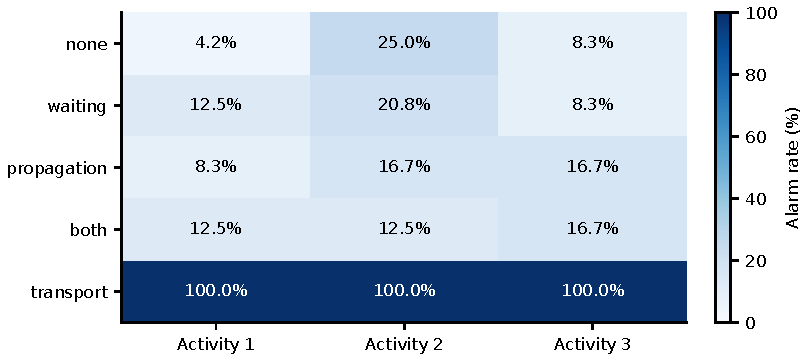
\includegraphics[width=.83\linewidth]{stress_alarms.pdf}
\caption{Full-model post-observation alarm rates on synthetic worlds. The no-shift row is a false-alarm control. Good detection of a large cancellation shock coexists with weak detection of waiting and propagation shifts. Intervals appear in Table~\ref{tab:stress}.}
\label{fig:stress}
\end{figure}
The original evaluator's diagnostic requires both low epistemic variance and RMSE above $0.08$. It never triggers for the waiting and propagation perturbations in this supplement. Table~\ref{tab:stress_magnitude} reports actual truth displacement: the waiting perturbation is small in some templates, so non-detection is not evidence of equal failure severity across shifts. Both diagnostics use realized outcomes and are not advance warnings. Shared agreement among misspecified candidates cannot, by itself, identify a missing rule.

\subsection{RQ2: What improves evidence efficiency, and what is accelerated?}
The original development AUC decreases from \InitialDev\ to \FinalDev, a \DevReduction\% reduction after adaptive selection on the same development set. The frozen test AUC is \TestAUC. This is evidence for the selected predictor on the fixed synthetic evaluation, not a percentage improvement over an external state of the art. The independent-world macro result is a different statistic and must not be substituted for the pooled test score.

Table~\ref{tab:acquisition_original} and the top row of Figure~\ref{fig:curves} show the original comparison. The lower Full curve includes the benefit of evolved calibration, whereas the other selectors start from uniform compatible weights. Under the matched-prior comparison in Table~\ref{tab:acquisition_matched}, the apparent acquisition advantage disappears. Matched-prior Random has macro AUC \MacroRandom, slightly below Full's \MacroFull. The differences are very small, and the near-flat curves indicate that the initially concentrated weights largely determine prediction. These controls prevent attributing calibration gains to the query criterion.
\begin{table}[tbp]
\centering
\caption{Original comparison: calibration and acquisition both vary. Activity AUC $\times10^3$ with 95\% world-bootstrap intervals; 24 worlds, fixed training data, evidence and templates.}
\label{tab:acquisition_original}
\scriptsize
\setlength{\tabcolsep}{3pt}
\begin{tabular}{lrrr}
\toprule
Method & Activity 1 & Activity 2 & Activity 3 \\
\midrule
Random & 17.82 [17.23, 18.39] & 19.03 [18.10, 20.01] & 14.96 [14.46, 15.44] \\
Entropy & 12.94 [12.27, 13.64] & 10.15 [9.21, 11.16] & 8.19 [7.32, 9.14] \\
ParamIG & 12.98 [12.34, 13.68] & 10.80 [10.06, 11.59] & 8.56 [7.50, 9.73] \\
Standard OED & 23.59 [22.32, 24.75] & 27.44 [24.79, 30.05] & 21.58 [19.34, 23.61] \\
Full & 4.19 [3.38, 5.07] & 10.85 [8.78, 12.85] & 6.15 [3.98, 8.65] \\
\bottomrule
\end{tabular}
\end{table}

\begin{table}[tbp]
\centering
\caption{Controlled acquisition comparison: all methods use the evolved prior. Activity AUC $\times10^3$ with 95\% world-bootstrap intervals; 24 worlds, fixed training data, evidence and templates.}
\label{tab:acquisition_matched}
\scriptsize
\setlength{\tabcolsep}{3pt}
\begin{tabular}{lrrr}
\toprule
Method & Activity 1 & Activity 2 & Activity 3 \\
\midrule
Matched-prior Random & 4.19 [3.38, 5.07] & 10.84 [8.77, 12.84] & 6.15 [3.98, 8.65] \\
Matched-prior Entropy & 4.19 [3.38, 5.07] & 10.85 [8.78, 12.85] & 6.15 [3.98, 8.65] \\
Matched-prior ParamIG & 4.19 [3.38, 5.07] & 10.85 [8.78, 12.85] & 6.15 [3.98, 8.65] \\
Matched-prior Standard OED & 4.19 [3.38, 5.07] & 10.85 [8.78, 12.85] & 6.15 [3.98, 8.65] \\
Full & 4.19 [3.38, 5.07] & 10.85 [8.78, 12.85] & 6.15 [3.98, 8.65] \\
\bottomrule
\end{tabular}
\end{table}

\begin{figure}[tbp]
\centering
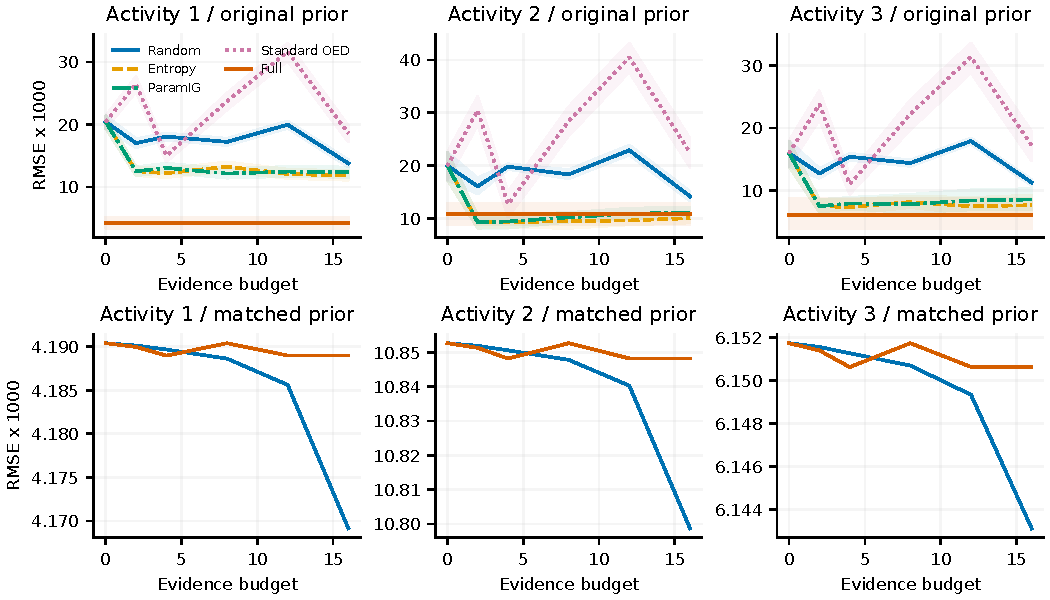
\includegraphics[width=\linewidth]{budget_curves.pdf}
\caption{Synthetic budget--trajectory error curves, reported separately by activity. Top: original calibration policies with conditional 95\% world-bootstrap shading. Bottom: all selectors share the evolved prior; curves nearly coincide. Bottom-row axes retain absolute values but use different scales, so their tiny variations should not be compared visually with top-row effect sizes.}
\label{fig:curves}
\end{figure}

\paragraph{Scoring microbenchmark.}
We compare covariance scoring with explicit enumeration of both binary outcomes, using identical candidates, cached predictions, probabilities, and costs. Ten GPU-synchronized timing pairs alternate execution order. Table~\ref{tab:timing} reports median per-pair speedups of \FrozenSpeed$\times$ under frozen weights and \UniformSpeed$\times$ under uniform compatible weights, with maximum score residuals. Figure~\ref{fig:evolution} displays the raw timings. The reference is the supplied loop-based enumeration implementation; a fully vectorized enumerator can share much of the same work. Accordingly, these measurements establish a local implementation advantage, not a universal speedup over optimized OED or an asymptotic improvement.
\begin{table}[tbp]
\centering
\caption{Ten synchronized, alternating-order GPU timing pairs. Median ratios are computed per pair; they need not equal the ratio of marginal medians.}
\label{tab:timing}
\scriptsize
\setlength{\tabcolsep}{3pt}
\begin{tabular}{lrrrr}
\toprule
Prior & Cov. (ms) & Enum. (ms) & Median ratio & Max. difference \\
\midrule
frozen & 0.773 & 178.17 & 217.95 & 9.08e-16 \\
uniform compatible & 0.747 & 191.85 & 275.16 & 1.38e-10 \\
\bottomrule
\end{tabular}
\end{table}

The canonical full frozen evaluation takes \TestRuntime\ seconds and reports \TestVRAM\ MB of peak allocated PyTorch GPU memory on an RTX 4060 Laptop GPU. These figures concern cached evaluation, excluding offline cache generation and graphics-driver memory. The development trials range from roughly four to nine seconds. Small cached evaluations are feasible on 8 GB VRAM, but this does not demonstrate equivalent scaling for larger populations or richer mechanism banks.

\subsection{RQ3: Which changes survive controlled ablation?}
Table~\ref{tab:ablations} compares the full model with four requested removals and a matched point estimate. Removing the combination target or batch conditioning leaves the aggregate results unchanged. This is consistent with near-single-mechanism weights: altering which evidence is chosen has little effect if the likelihood cannot move substantial mass. Removing sharing worsens results, but its bank uses independent per-event parameter permutations and changes the prior and hypothesis space. The comparison is informative about that implementation, not a pure causal estimate of the benefit of sharing.
\begin{table}[tbp]
\centering
\caption{Frozen-method ablations. Asterisks identify changes that also alter the prior or point-selection objective. Activity AUC $\times10^3$ with 95\% world-bootstrap intervals; 24 worlds, fixed training data, evidence and templates.}
\label{tab:ablations}
\scriptsize
\setlength{\tabcolsep}{3pt}
\begin{tabular}{lrrr}
\toprule
Method & Activity 1 & Activity 2 & Activity 3 \\
\midrule
Full & 4.19 [3.38, 5.07] & 10.85 [8.78, 12.85] & 6.15 [3.98, 8.65] \\
Without sharing* & 47.19 [45.23, 49.01] & 21.17 [18.72, 23.61] & 51.11 [48.60, 53.35] \\
Without combination target & 4.19 [3.38, 5.07] & 10.85 [8.78, 12.85] & 6.15 [3.98, 8.65] \\
Original single point* & 5.42 [4.71, 6.08] & 7.54 [5.92, 9.35] & 7.37 [5.78, 8.95] \\
Matched MAP & 4.19 [3.38, 5.07] & 10.85 [8.78, 12.85] & 6.15 [3.99, 8.65] \\
Without batch conditioning & 4.19 [3.38, 5.07] & 10.85 [8.78, 12.85] & 6.15 [3.98, 8.65] \\
\bottomrule
\end{tabular}
\end{table}


The development history explains the concentration. Rounds 1--7 introduce trajectory weighting and progressively narrow its kernel. Round 30 replaces average historical error with worst-event error. Round 38 narrows the kernel again, but the accepted improvement is only around $10^{-7}$ and should not be presented as a performance leap. Round 58 introduces the noise normalization in Eq.~\eqref{eq:distance}; it produces the largest later improvement. These sequential decisions are not independent ablations, since each accepted change becomes the next parent. All 60 scores and decisions appear in Appendix~\ref{app:trials}.

The aggregate objective also trades off against process prediction: development Brier worsens from \DevBrierStart\ to \DevBrierEnd, and frozen-test Brier is \TestBrier. Frozen-test pointwise coverage is \TestCoverage\% with mean width \TestWidth. High marginal coverage does not establish identified mechanisms or calibrated out-of-model uncertainty. The independent-world uncertainty table (Table~\ref{tab:uncertainty}) separates epistemic and aleatoric contributions; the former is tiny relative to the latter under the selected weights.
\begin{figure}[tbp]
\centering
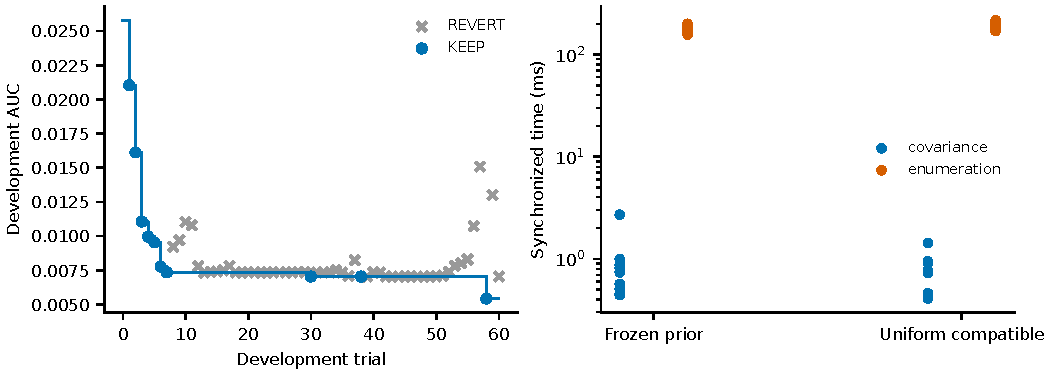
\includegraphics[width=\linewidth]{evolution_timing.pdf}
\caption{Left: all 60 development candidates and the retained-score trajectory. Reverted trials remain visible. Right: all ten timing pairs for each prior; the logarithmic axis distinguishes covariance and explicit enumeration costs without treating timing repetitions as independent activity replicates.}
\label{fig:evolution}
\end{figure}

\section{Discussion and related work}
\subsection{Relationship to calibration and experimental design}
\paragraph{Calibration under non-identifiability.}
Bayesian computer-model calibration distinguishes parameter uncertainty from model discrepancy \citep{kennedy2001}. Eligibility-set calibration already addresses non-identifiability in multi-agent simulators and combines distributional comparison with Bayesian optimization \citep{bai2022}. Our empirical process/trajectory gates are simpler and lack their statistical test interpretation. Bayesian optimization for likelihood-free inference allocates expensive simulator evaluations \citep{gutmann2016}; our acquisition instead allocates access to process records after rollouts have been cached. These are different resource decisions. Set calibration itself is therefore not a novelty claim. The contribution lies in its explicit coupling to stage-level evidence opportunities, composed target trajectories, and an auditable evaluation of when that coupling becomes ineffective.

\paragraph{Prediction-directed acquisition.}
Variance-based active learning has a long history \citep{cohn1996}, and Bayesian design provides a decision-theoretic framework for utility-dependent data acquisition \citep{chaloner1995}. Goal-oriented OED targets predictive quantities rather than all parameter uncertainty \citep{attia2018,zhong2026}. Our squared-covariance score is a finite binary-observation specialization of that perspective, using a variance utility rather than predictive information gain. A record with high entropy can still have zero value if every mechanism assigns it the same probability or if it is uncorrelated with the probe prediction. The relevant practical decisions are the validity of stage likelihoods, the target probe distribution, numerical support preservation, and computation reuse. The current evidence supports the last of these most clearly.

\paragraph{Social simulation systems.}
CALM combines calibrated stochastic choice with activity-based traveler simulation \citep{cheng2026}; it concerns a specific empirical mobility setting rather than the finite process-record acquisition problem studied here. SocioVerse2 develops longitudinal simulation and research loops for social systems \citep{zhang2026}. Large Population Models emphasize population-scale behavior and interactions \citep{chopra2025}. These systems motivate reusable interfaces between mechanisms, observations, and collective outcomes. They are not empirical baselines in this paper, and an adapter bearing a benchmark name is not a reproduction of their evaluation. The proposal's broader aim of recovering individual dynamics from macro observations is also reflected in macro2mind \citep{macro2mind2026}; we do not implement or compare that model. Real-domain comparisons would require compatible observation opportunities, licensed data, and a named, frozen scoring protocol.

\subsection{Scope, boundary conditions, and failure modes}
\label{sec:boundaries}
\paragraph{Concentration removes the signal used by acquisition.}
As $w$ approaches a point mass, $\Cov_w(p_r,Z)\to0$ for every record and hence $A_r(w)\to0$. A large hard-compatible set is therefore not sufficient to preserve epistemic uncertainty. The chosen small kernel width and finite-precision softmax jointly restrict effective support. Posterior updates cannot recover candidates with exactly zero mass. The observed absence of acquisition gains is consistent with this limit, but proving its quantitative contribution would require controlled interventions beyond this frozen study.

\paragraph{Why plausible development changes failed.}
Wider kernels in rounds 8--9 and 36--37 were reverted: keeping more candidate mass increased prediction error on the chosen development objective. Mixing in uniform weight in rounds 14--17 and 50--53 also failed to improve it. These outcomes distinguish numerical diversity from accurate uncertainty; they do not prove that diverse sets are generally inferior. Stronger evidence likelihoods at temperatures $0.05$ and $0.1$ worsened results in rounds 10--11, consistent with noisy binary evidence exerting excessive influence under a mismatched finite bank. Later temperature changes had only negligible effects once the mixture was already concentrated.

Rounds 18--23 added process Brier energy with almost no change in the retained behavior. Rounds 24--29 changed channel weights without exceeding the acceptance threshold. Alternative worst-channel, absolute, Huber, trimmed, and late-time objectives in rounds 31--35 did not improve the score. These losses encode different notions of fit; none is a universally valid robustness correction. Probe-coordinate rescaling in rounds 42--45 produced identical AUC, an especially direct warning against describing those rejected ideas as innovations in the final method. Seed-marginalized kernels in rounds 54--57 performed worse, but this changed both the calibration construction and kernel scale, so the result does not show that modeling randomness is harmful. Finally, raising the variance floor in rounds 59--60 reversed the benefit of round 58. Sensitivity to this regularizer is a limitation, not evidence that the selected value transfers to new domains.

\paragraph{Batch conditioning does not imply submodularity.}
Adaptive-submodularity guarantees require a diminishing-returns property \citep{golovin2011}. Our objective does not satisfy it in general. Consider a mechanism indexed by two independent fair bits $(U,V)$, target $Z=U\oplus V$, and two noiseless queries revealing $U$ and $V$. Either query alone leaves target variance unchanged, while both determine $Z$. The marginal value of the second query increases after acquiring the first, violating diminishing returns, even though query outcomes are deterministic and thus conditionally independent given the mechanism. This analytical counterexample explains why exact fantasy averaging is described as greedy conditional acquisition, without a generic approximation guarantee.

\paragraph{Agreement can coexist with arbitrary misspecification.}
Suppose all candidates predict $z_0$ while an omitted environmental rule makes reality $z_0+\Delta$. Every epistemic covariance and acquisition score is zero, while mean squared error is $\|\Delta\|^2/D$. The variance-reduction identity remains valid internally. It cannot discover a mechanism absent from the candidate class, and broad aleatoric intervals may conceal weak shifts. Post-observation residual checks provide a different source of evidence, but the tested thresholds have neither calibrated false-positive control nor advance-warning guarantees. Candidate expansion and explicit discrepancy models are possible remedies, not implemented successes.

\paragraph{What the current evidence does and does not support.}
The same development split selected 60 candidates; reporting its best score without the full search history would overstate validation. The test evaluation and independent-world extension strengthen reproducibility but retain fixed templates, training data, evidence, and a small finite mechanism bank. No confidence interval here covers uncertainty over human populations or over the search procedure itself. The Round-2 extension in Section~\ref{sec:round2} partially addresses this issue with fresh acquisition cohorts and a new sealed holdout. Further evaluation should vary event designs, historical datasets and query pools, include same-prior optimized OED, and test whether the noncollapsed acquisition benefit persists outside the constructed stress setting. It would also isolate sharing from prior changes and validate observation models before using real behavioral records.

\subsection{Conclusion}
The study makes a budgeted process-evidence loop explicit and inexpensive to execute, with complete-path prediction and separable uncertainty terms. Its strongest empirical lesson is that successful aggregate calibration can eliminate the mechanism disagreement on which active evidence selection depends. The frozen implementation improves synthetic trajectory prediction and accelerates a reference scoring calculation, but the V1 matched controls do not establish an acquisition or set-retention advantage. The separate V2 stress test restores an acquisition advantage over matched Random and Entropy while tying ParamIG; its constructed nuisance pool and inactive batch ablation limit the claim. Treating that distinction as a result yields a more useful foundation for compositional social simulation than an unsupported claim of mechanism identification or external benchmark superiority.

\bibliographystyle{plainnat}
\bibliography{references}
\clearpage
\appendix
\section{Additional results and audit trail}
\label{app:results}
All tables below are generated from the same sealed result files as the main text. They are not additional tuning runs. Table~\ref{tab:golden} retains the original evaluator's pooled metric, whereas the other activity tables use independent-world replication. The distinction prevents a change in aggregation from being mistaken for a change in performance.
\begin{table}[H]
\centering
\caption{Original frozen test cache, descriptive results. Random is averaged over its three query repetitions. These interacting activities do not constitute independent replicates.}
\label{tab:golden}
\scriptsize
\setlength{\tabcolsep}{3pt}
\begin{tabular}{lrrrrr}
\toprule
Method & Pooled AUC & Brier & NLL & Coverage & Width \\
\midrule
Random & 0.017980 & 0.1957 & 0.5775 & 1.0000 & 0.0666 \\
Entropy & 0.011052 & 0.1862 & 0.5572 & 1.0000 & 0.0691 \\
ParamIG & 0.011017 & 0.1860 & 0.5618 & 1.0000 & 0.0679 \\
Standard OED & 0.025494 & 0.2086 & 0.6021 & 1.0000 & 0.0666 \\
Full & 0.006916 & 0.2459 & 0.6811 & 0.9792 & 0.0304 \\
Simple statistics & 0.023584 & 0.3026 & 0.8458 & 0.8125 & 0.0318 \\
Uncalibrated & 0.017490 & 0.2144 & 0.6139 & 1.0000 & 0.0896 \\
Process only & 0.019877 & 0.2238 & 0.6328 & 1.0000 & 0.0769 \\
Trajectory only & 0.018181 & 0.2202 & 0.6253 & 1.0000 & 0.0804 \\
Passive V1 & 0.019877 & 0.2238 & 0.6328 & 1.0000 & 0.0769 \\
Without sharing* & 0.051271 & 0.2050 & 0.6108 & 0.6146 & 0.0360 \\
Without combination target & 0.006916 & 0.2459 & 0.6811 & 0.9792 & 0.0304 \\
Original single point* & 0.008321 & 0.2513 & 0.7070 & 0.9479 & 0.0291 \\
\bottomrule
\end{tabular}
\end{table}

\begin{table}[H]
\centering
\caption{Passive calibration baselines. These rows acquire no additional evidence. Activity AUC $\times10^3$ with 95\% world-bootstrap intervals; 24 worlds, fixed training data, evidence and templates.}
\label{tab:calibration}
\scriptsize
\setlength{\tabcolsep}{3pt}
\begin{tabular}{lrrr}
\toprule
Method & Activity 1 & Activity 2 & Activity 3 \\
\midrule
Simple statistics & 24.05 [23.81, 24.30] & 32.30 [30.39, 34.18] & 18.84 [18.07, 19.77] \\
Uncalibrated & 19.99 [19.34, 20.63] & 17.08 [15.25, 18.87] & 13.81 [12.79, 14.89] \\
Process only & 20.43 [19.38, 21.40] & 19.94 [17.30, 22.45] & 15.96 [13.85, 17.89] \\
Trajectory only & 19.56 [18.65, 20.40] & 17.66 [15.15, 20.03] & 14.28 [12.53, 15.93] \\
Passive V1 & 20.43 [19.38, 21.40] & 19.94 [17.30, 22.45] & 15.96 [13.85, 17.89] \\
\bottomrule
\end{tabular}
\end{table}

\begin{table}[H]
\centering
\caption{Paired activity AUC differences $\times10^6$ with 95\% world-bootstrap intervals. Positive favors Full; tiny differences are not necessarily practically meaningful.}
\label{tab:paired}
\scriptsize
\setlength{\tabcolsep}{3pt}
\begin{tabular}{lrrr}
\toprule
Comparator minus Full & Activity 1 & Activity 2 & Activity 3 \\
\midrule
Matched MAP & 1.19 [0.62, 1.84] & 3.72 [2.22, 5.21] & 0.92 [-0.18, 2.07] \\
Matched-prior Random & -3.61 [-5.60, -1.70] & -8.86 [-13.65, -3.83] & -1.38 [-5.02, 2.14] \\
Without combination target & 0.00 [0.00, 0.00] & 0.00 [0.00, 0.00] & 0.00 [0.00, 0.00] \\
Without batch conditioning & 0.00 [0.00, 0.00] & 0.00 [0.00, 0.00] & 0.00 [0.00, 0.00] \\
\bottomrule
\end{tabular}
\end{table}

\begin{table}[H]
\centering
\caption{Final-budget uncertainty: means and 95\% world-bootstrap intervals. Coverage concerns pointwise 90\% predictive intervals.}
\label{tab:uncertainty}
\scriptsize
\setlength{\tabcolsep}{3pt}
\begin{tabular}{lrrr}
\toprule
Quantity & Activity 1 & Activity 2 & Activity 3 \\
\midrule
Coverage (percent) & 94.0 [91.9, 95.9] & 90.8 [87.9, 93.7] & 92.5 [89.0, 95.4] \\
Interval width (fraction) & 0.0167 [0.0135, 0.0202] & 0.0349 [0.0313, 0.0387] & 0.0304 [0.0277, 0.0333] \\
Epistemic variance x 1e8 & 3.41 [2.65, 4.22] & 9.71 [6.72, 13.12] & 4.45 [3.01, 6.14] \\
Aleatoric variance x 1e4 & 0.91 [0.69, 1.14] & 3.04 [2.48, 3.69] & 2.42 [2.05, 2.80] \\
\bottomrule
\end{tabular}
\end{table}

\begin{table}[H]
\centering
\caption{True trajectory displacement relative to the no-shift world, RMSE $\times10^3$. Reported separately to distinguish weak perturbations from insensitive detection.}
\label{tab:stress_magnitude}
\scriptsize
\setlength{\tabcolsep}{3pt}
\begin{tabular}{lrrr}
\toprule
Truth rule & Activity 1 & Activity 2 & Activity 3 \\
\midrule
none & 0.00 [0.00, 0.00] & 0.00 [0.00, 0.00] & 0.00 [0.00, 0.00] \\
waiting & 3.55 [3.18, 3.93] & 0.61 [0.28, 0.97] & 0.38 [0.18, 0.61] \\
propagation & 7.92 [7.35, 8.54] & 10.16 [9.17, 11.16] & 19.64 [18.42, 20.70] \\
both & 7.37 [6.75, 8.07] & 10.15 [9.17, 11.15] & 19.21 [17.98, 20.30] \\
transport & 59.52 [58.46, 60.48] & 74.78 [72.55, 76.86] & 53.31 [51.58, 54.89] \\
\bottomrule
\end{tabular}
\end{table}

\FloatBarrier
\section{Reproduction and evidence provenance}
\label{app:reproduction}
The frozen algorithm is commit \texttt{eb641c2}; its SHA-256 is recorded in the machine-readable artifact manifest. The manuscript generator verifies this hash before producing figures. It reads the canonical frozen evaluation, the fixed 24-world supplement, the audited candidate ledger, and the campaign summary. All other root-level JSON results are inventoried with hashes and retained as historical or reproduction runs, rather than selected by test performance. The candidate audit reconciles decision rows with evaluation rows by run identifier and verifies their Git sources. Thus 60 candidates, not the number of ledger lines, define the search budget.

The release separates environment preparation, the fixed evaluator, the sole evolvable algorithm file, and the search controller. The present manuscript changes none of them. The original cache contains labels in the same local process; source checks and API conventions provide auditability, not an adversarially secure holdout. A deployment with sensitive observations would require a separate permission-controlled evaluation service.

To rebuild the figures and PDF, run \texttt{python paper/generate\_artifacts.py}, followed by \texttt{python paper/build.py}, from the repository root in the supplied research environment. The latter invokes pdfLaTeX and BibTeX from the paper directory and checks the final log for unresolved references and layout warnings. The standalone paper source directory also supports conventional pdfLaTeX--BibTeX compilation. The research reproduction script at the root is separate: it can rerun the sealed synthetic experiments but is not required to typeset the manuscript. Cached evaluation excludes offline simulation cost; Table~\ref{tab:timing} additionally excludes cache loading, calibration, posterior prediction, and figure generation.

No human participants were recruited and no real student records were used. The executable social model represents a constructed resource-participation process. Its parameters must not be interpreted as estimates of individual psychological traits. The SocioVerse and SocialSim integration materials are interface preparation, not evidence of external validity or an official leaderboard submission.

\section{Complete development decisions}
\label{app:trials}
Table~\ref{tab:alltrials} reports every accepted and rejected candidate in chronological order. Rejection includes changes that were numerically indistinguishable or smaller than the predeclared acceptance threshold; it does not always mean a substantial deterioration. Hypotheses, full source hashes, and exact candidate files remain in the repository's evolution audit. These observations explain the selected implementation but do not replace a new independent comparison of the corresponding mathematical choices.
\footnotesize
\begin{longtable}{rrrll}
\caption{All 60 audited candidates. Development scores are adaptively selected, not independent validation.}\label{tab:alltrials}\\
\toprule Round & Dev AUC & Parent AUC & Decision & Commit \\ \midrule\endfirsthead
\toprule Round & Dev AUC & Parent AUC & Decision & Commit \\ \midrule\endhead
1 & 0.02103133 & 0.02579135 & KEEP & \texttt{9004e27} \\
2 & 0.01612103 & 0.02103133 & KEEP & \texttt{6bb9ddb} \\
3 & 0.01106276 & 0.01612103 & KEEP & \texttt{73386c1} \\
4 & 0.00996100 & 0.01106276 & KEEP & \texttt{728d215} \\
5 & 0.00954380 & 0.00996100 & KEEP & \texttt{ba8b306} \\
6 & 0.00776780 & 0.00954380 & KEEP & \texttt{d5e58c8} \\
7 & 0.00734499 & 0.00776780 & KEEP & \texttt{ef86a46} \\
8 & 0.00921580 & 0.00734499 & REVERT & \texttt{73f16c4} \\
9 & 0.00969213 & 0.00734499 & REVERT & \texttt{478719a} \\
10 & 0.01102639 & 0.00734499 & REVERT & \texttt{05f5dcf} \\
11 & 0.01080275 & 0.00734499 & REVERT & \texttt{b4c4fca} \\
12 & 0.00780723 & 0.00734499 & REVERT & \texttt{3088266} \\
13 & 0.00734522 & 0.00734499 & REVERT & \texttt{b4fe2a0} \\
14 & 0.00735953 & 0.00734499 & REVERT & \texttt{3df239c} \\
15 & 0.00741803 & 0.00734499 & REVERT & \texttt{25afcf5} \\
16 & 0.00749185 & 0.00734499 & REVERT & \texttt{4b1e757} \\
17 & 0.00779464 & 0.00734499 & REVERT & \texttt{bff1fc7} \\
18 & 0.00734499 & 0.00734499 & REVERT & \texttt{ff4fbbf} \\
19 & 0.00734499 & 0.00734499 & REVERT & \texttt{dbba10b} \\
20 & 0.00734499 & 0.00734499 & REVERT & \texttt{e09f641} \\
21 & 0.00734499 & 0.00734499 & REVERT & \texttt{35d2997} \\
22 & 0.00734499 & 0.00734499 & REVERT & \texttt{99e2128} \\
23 & 0.00734499 & 0.00734499 & REVERT & \texttt{0a72bd0} \\
24 & 0.00734499 & 0.00734499 & REVERT & \texttt{2721c24} \\
25 & 0.00737358 & 0.00734499 & REVERT & \texttt{6ebab02} \\
26 & 0.00734499 & 0.00734499 & REVERT & \texttt{0cae7ed} \\
27 & 0.00734532 & 0.00734499 & REVERT & \texttt{7292291} \\
28 & 0.00739139 & 0.00734499 & REVERT & \texttt{037df88} \\
29 & 0.00734499 & 0.00734499 & REVERT & \texttt{d83f2e1} \\
30 & 0.00704311 & 0.00734499 & KEEP & \texttt{98d6fb0} \\
31 & 0.00734499 & 0.00704311 & REVERT & \texttt{bc4d425} \\
32 & 0.00738014 & 0.00704311 & REVERT & \texttt{55a1b8f} \\
33 & 0.00734523 & 0.00704311 & REVERT & \texttt{f29e090} \\
34 & 0.00751265 & 0.00704311 & REVERT & \texttt{07fe993} \\
35 & 0.00734499 & 0.00704311 & REVERT & \texttt{4e8b0ca} \\
36 & 0.00706689 & 0.00704311 & REVERT & \texttt{f929916} \\
37 & 0.00823951 & 0.00704311 & REVERT & \texttt{f7fee7e} \\
38 & 0.00704303 & 0.00704311 & KEEP & \texttt{6a44dfc} \\
39 & 0.00704303 & 0.00704303 & REVERT & \texttt{9007fd6} \\
40 & 0.00734499 & 0.00704303 & REVERT & \texttt{4612d6b} \\
41 & 0.00734499 & 0.00704303 & REVERT & \texttt{7702d9c} \\
42 & 0.00704303 & 0.00704303 & REVERT & \texttt{6ff50b7} \\
43 & 0.00704303 & 0.00704303 & REVERT & \texttt{eb9bd17} \\
44 & 0.00704303 & 0.00704303 & REVERT & \texttt{8361b7a} \\
45 & 0.00704303 & 0.00704303 & REVERT & \texttt{be36314} \\
46 & 0.00704304 & 0.00704303 & REVERT & \texttt{871658d} \\
47 & 0.00704303 & 0.00704303 & REVERT & \texttt{f7077c6} \\
48 & 0.00704303 & 0.00704303 & REVERT & \texttt{320da5d} \\
49 & 0.00704303 & 0.00704303 & REVERT & \texttt{945ecb9} \\
50 & 0.00704964 & 0.00704303 & REVERT & \texttt{34ebfd4} \\
51 & 0.00711002 & 0.00704303 & REVERT & \texttt{72363f1} \\
52 & 0.00739650 & 0.00704303 & REVERT & \texttt{39cf814} \\
53 & 0.00782675 & 0.00704303 & REVERT & \texttt{307cd3d} \\
54 & 0.00802215 & 0.00704303 & REVERT & \texttt{c34f927} \\
55 & 0.00829448 & 0.00704303 & REVERT & \texttt{a7e246c} \\
56 & 0.01073823 & 0.00704303 & REVERT & \texttt{3c56dc0} \\
57 & 0.01507502 & 0.00704303 & REVERT & \texttt{b4ee347} \\
58 & 0.00543199 & 0.00704303 & KEEP & \texttt{eb641c2} \\
59 & 0.01300248 & 0.00543199 & REVERT & \texttt{1b4c940} \\
60 & 0.00704303 & 0.00543199 & REVERT & \texttt{135f671} \\
\bottomrule
\end{longtable}

\end{document}
